

\begin{figure}[htbp]
\centering
\definecolor{colHeat}{RGB}{55,138,221}
\definecolor{colLight}{RGB}{239,159,39}
\definecolor{colEMF}{RGB}{151,196,89}
\definecolor{colRF}{RGB}{212,83,126}
\definecolor{colMech}{RGB}{127,119,221}
\definecolor{colChem}{RGB}{136,135,128}
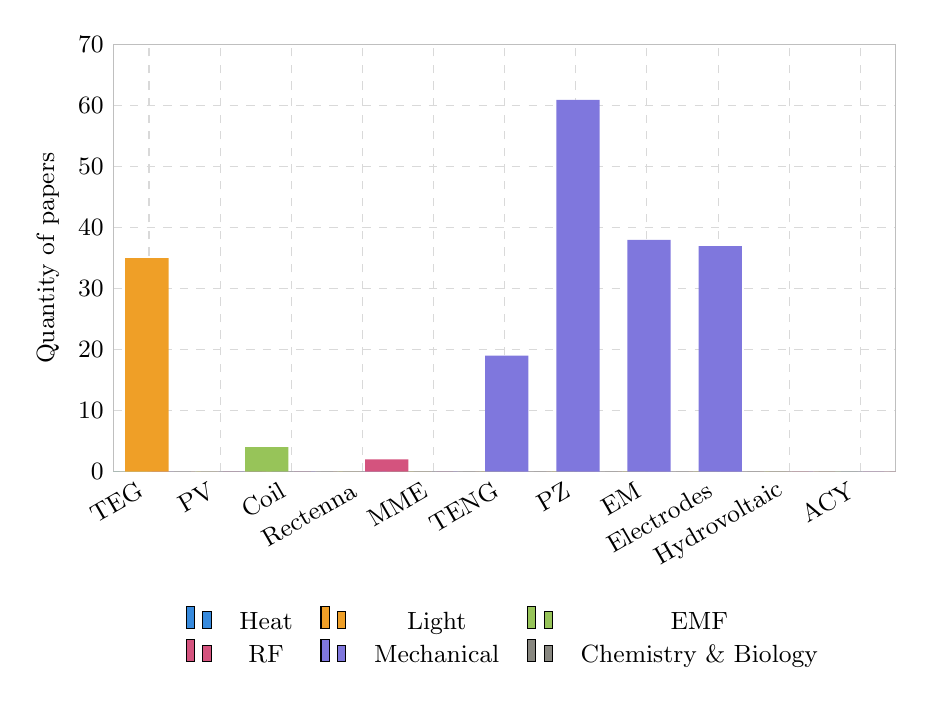
\begin{tikzpicture}
\begin{axis}[
    ybar,
    bar width        = 0.55cm,
    width            = 0.95\textwidth,
    height           = 7cm,
    enlarge x limits = 0.05,
    ylabel           = {Quantity of papers},
    ylabel style     = {font=\small},
    symbolic x coords = {TEG, PV, Coil, Rectenna, MME,
                          TENG, PZ, EM, Electrodes, Hydrovoltaic, ACY},
    xtick            = data,
    xticklabel style = {font=\small, rotate=30, anchor=east},
    ymin = 0, ymax   = 70,
    ytick            = {0,10,20,30,40,50,60,70},
    yticklabel style = {font=\small},
    grid             = major,
    grid style       = {dashed, gray!30},
    axis line style  = {gray!50},
    tick style       = {draw=none},
    legend style     = {
        at={(0.5,-0.30)},
        anchor=north,
        legend columns=3,
        font=\small,
        draw=none,
        column sep=0.8em
    },
]

\addplot[fill=colHeat, draw=none] coordinates {
    (TEG,24)(PV,0)(Coil,0)(Rectenna,0)(MME,0)
    (TENG,0)(PZ,0)(EM,0)(Electrodes,0)(Hydrovoltaic,0)(ACY,0)};
\addlegendentry{Heat}

\addplot[fill=colLight, draw=none] coordinates {
    (TEG,0)(PV,35)(Coil,0)(Rectenna,0)(MME,0)
    (TENG,0)(PZ,0)(EM,0)(Electrodes,0)(Hydrovoltaic,0)(ACY,0)};
\addlegendentry{Light}

\addplot[fill=colEMF, draw=none] coordinates {
    (TEG,0)(PV,0)(Coil,4)(Rectenna,0)(MME,0)
    (TENG,0)(PZ,0)(EM,0)(Electrodes,0)(Hydrovoltaic,0)(ACY,0)};
\addlegendentry{EMF}

\addplot[fill=colRF, draw=none] coordinates {
    (TEG,0)(PV,0)(Coil,0)(Rectenna,2)(MME,0)
    (TENG,0)(PZ,0)(EM,0)(Electrodes,0)(Hydrovoltaic,0)(ACY,0)};
\addlegendentry{RF}

\addplot[fill=colMech, draw=none] coordinates {
    (TEG,0)(PV,0)(Coil,0)(Rectenna,0)(MME,19)
    (TENG,61)(PZ,38)(EM,37)(Electrodes,0)(Hydrovoltaic,0)(ACY,0)};
\addlegendentry{Mechanical}

\addplot[fill=colChem, draw=none] coordinates {
    (TEG,0)(PV,0)(Coil,0)(Rectenna,0)(MME,0)
    (TENG,0)(PZ,0)(EM,0)(Electrodes,0)(Hydrovoltaic,0)(ACY,0)};
\addlegendentry{Chemistry \& Biology}

\end{axis}
\end{tikzpicture}
\caption{Distribution of papers based on transducer type.
Adapted from \cite{leonavilaEnergyHarvestingTechniques2025}.}
\label{fig:transducer_distribution}
\end{figure}
